% don't remove the folling lines, and edit the defintion of \main if needed
\documentclass[../report.tex]{subfiles}
\providecommand{\main}{..}
\IfEq{\jobname}{\currfilebase}{\AtEndDocument{\biblio}}{}
% until here

%To have the comments written on the PDF: keep this macro
\newcommand{\commentsinout}[1]{#1}
%To have the comments hidden in the PDF: keep this macro
%\newcommand{\commentsinout}[1]{}

% this is a macro so you can make comments. See example below.
\newcommand{\KE}[1]{\commentsinout{{\bf{\color{brown} [KE: #1]}}}} % Comments by K. Ellis
\newcommand{\BH}[1]{\commentsinout{{\bf{\color{cyan} [BH: #1]}}}} % Comments by B. Heinemann
\newcommand{\FM}[1]{\commentsinout{{\bf{\color{orange} [FM: #1]}}}} % Comments by F. Maltoni
\newcommand{\AN}[1]{\commentsinout{{\bf{\color{teal} [AN: #1]}}}} % Comments by A. Nisati
\newcommand{\CW}[1]{\commentsinout{{\bf{\color{teal} [CW: #1]}}}} % Comments by A. Nisati

\begin{document}

\section{Astrophysical Probes of Dark Matter}


The understanding of the dark matter properties will demand signals from multiple experiments, together with compatibility with indirect measurements from DM annihilation products. This section  briefly reports on the status and prospects for DM Direct Detection (DD) and Indirect Detection (ID) searches, with emphasis on masses greater that about 1 GeV. For lower mass regimes see Sects.~4.5 and 5.3.

\subsection{Direct detection}


% start JRM
%\textit{Current results.} 
%Collider experiment searches have mostly excluded WIMP dark matter candidates with masses below 80 GeV, in minimal supersymmetry (SUSY) models. The ATLAS and CMS experiment limits on dark matter are highly competitive with existing and planned direct dark matter search experiments for very low ($<$10 GeV) WIMP masses, although there are model-specific assumptions (about, e.g.~the involved WIMP-nucleon couplings). The range of dark matter particle masses accessible at the LHC is limited by the total center of mass energy, which results in decreasing sensitivity for WIMP masses above a few hundred GeV. The WIMP mass coverage and interaction sensitivity of direct detection searches are thus highly complementary to those of the LHC, since direct detection has no similar kinematic limit on the maximum dark matter mass reach.
%
At present, direct detection searches have excluded spin-independent dark matter-nucleon cross sections as low as ~10$^{-46}$ cm$^2$ %\cite{Cui:2017kg,Aprile:2018ct}, 
shown as solid curves in Fig.~\ref{fig:sensitivity}, and spin-dependent cross sections as low as 10$^{-41}$ cm$^2$
%\cite{Amole:2017iz}.  
For interactions with heavy mediators, collider searches have broadly comparable sensitivity within the subset of models and parameters chosen in Chapter~\ref{chap:bsm};
%under specific model assumptions~\cite{Aaboud:2019yqu,currentCollider} 
%as illustrated  in Fig.~\ref{fig:sensitivity}; more detailed 
specific examples are shown in Sect.~\ref{subsec:complementarity_collider}.  The leading results in the 5 GeV range and below come from the DarkSide-50 LAr TPC low mass search and from cryogenic solid state detectors, while at higher masses from cryogenic noble liquids, led for the past decade by the pioneering XENON program at LNGS.  There have also been several experiments that are consistent with a dark matter signal, both from direct 
%\cite{Bernabei:2010gs, Aalseth:2014wc, Agnese:2013hy, Angloher:2012kl} 
and indirect
%\cite{Aguilar:2014cj,Ajello:2016ge} 
searches. These results demonstrate that confirmation by multiple experiments, with independent detection strategies and targets, is essential for a convincing discovery.
%
\begin{figure}[t]
\centering
  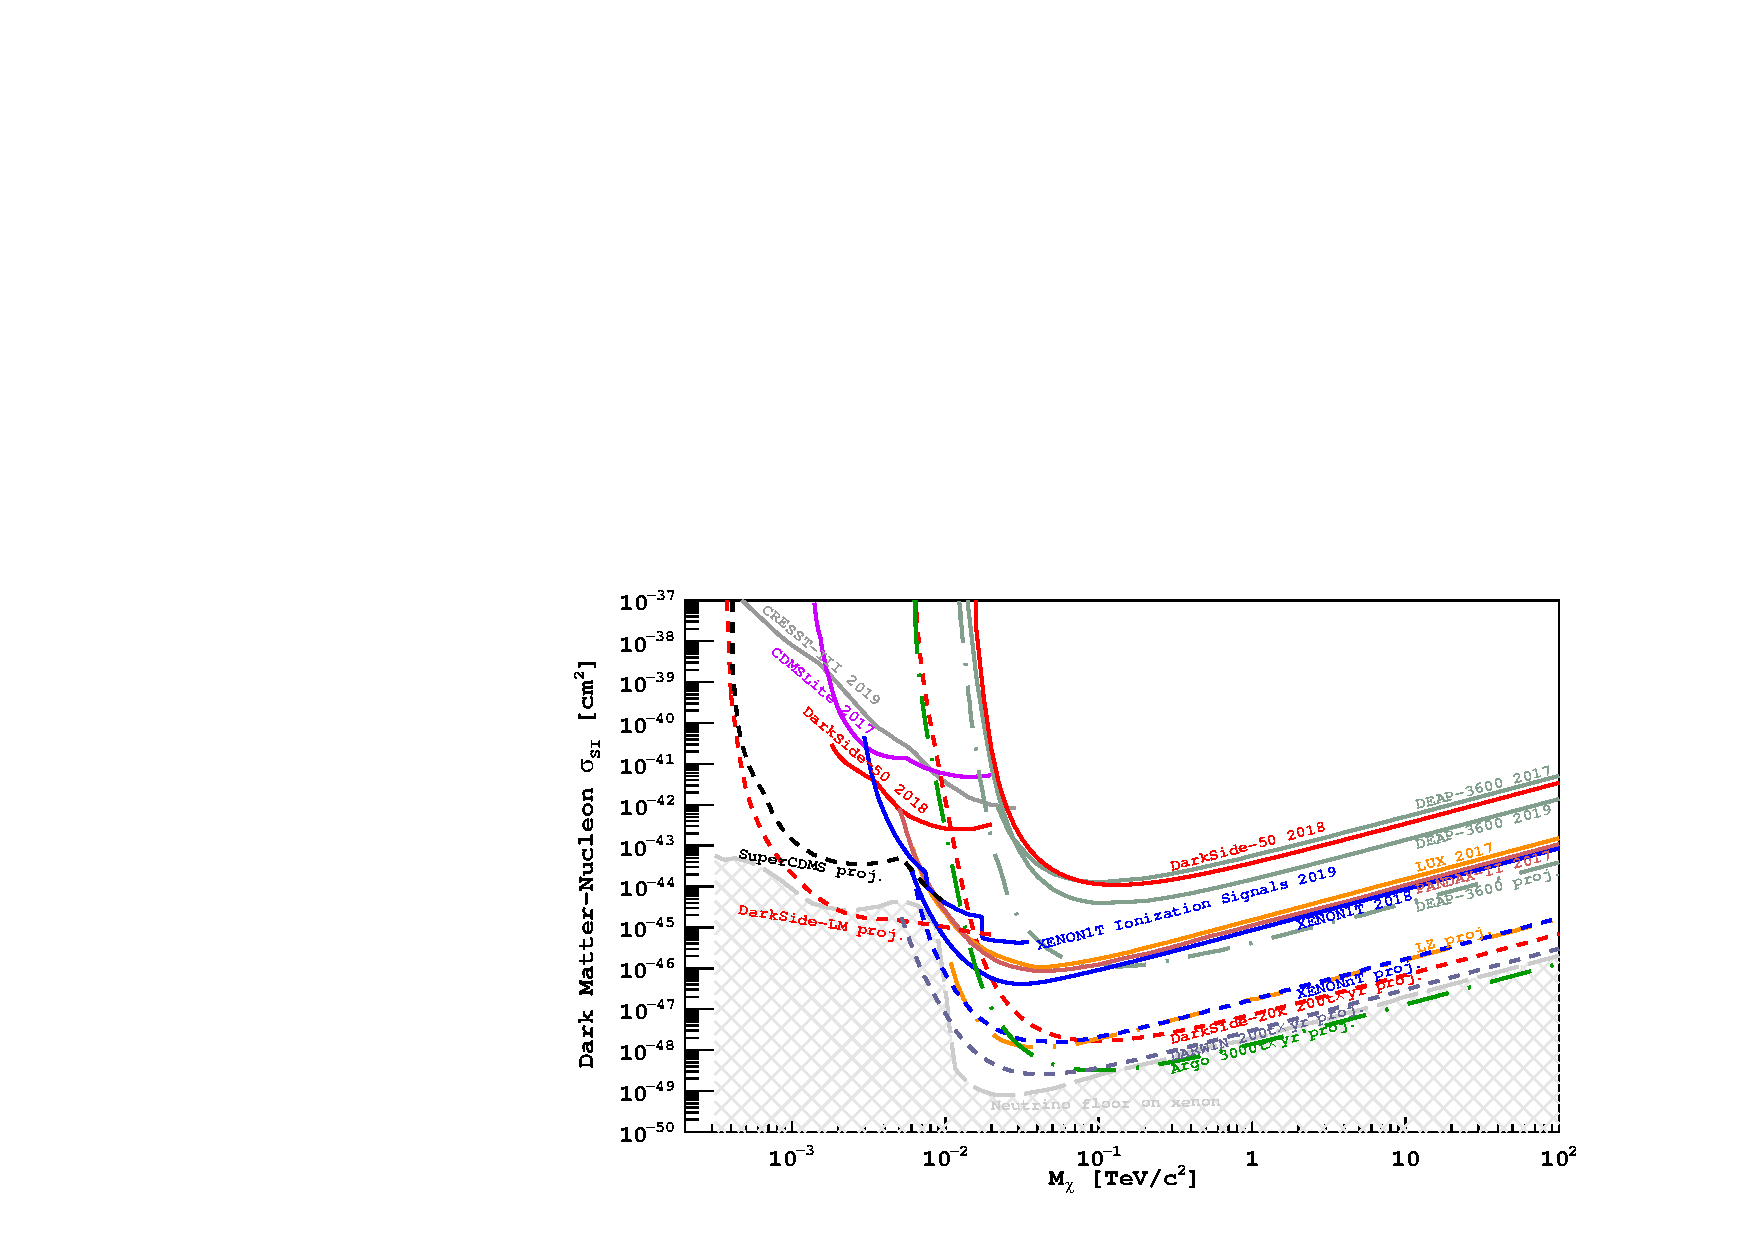
\includegraphics[width=0.78\linewidth,angle=0,origin=c]{Darkmatter/section1/img/CombinedExclusionLimits_nufloor_2.pdf}
 % \vspace{-3.5cm}
\caption{90\% C.L. exclusion limits showing leading results from direct detection (continuous lines, %Ref.~\cite{Angloher:2012kl,Akerib:2017kg,Cui:2017kg,Aprile:2018ct,PhysRevD.98.102006,Agnes:2018fg}) 
%and an indicative accelerator-based dark matter searches (region above the yellow line \cite{TheATLASCollaboration:2018to}) compared with 
Sensitivities of future Ge-, Xe-, and Ar-based direct searches are also shown with dashed lines. %, Ref.~\cite{Nelson:2014wy,Kudryavtsev:2015hy,Aprile:2015wv,Boulay:2017tn,Agnese:2017fn}). 
The neutrino floor curve follows the definition of Ref.~\cite{Billard:2014cx}. %The 95\% C.L. limit from the ATLAS Experiment is shown for a model in which Dirac-fermion WIMPs interact with ordinary matter via a vector mediator with benchmark coupling strengths to quarks, leptons and WIMPs of 0.25, 0.01, and 1, respectively ~\cite{Abercrombie:2015to}. 
}
\label{fig:sensitivity}
\end{figure}
%
%%%%%%%%%%%%%%%%%%%%%%%%%%%%%%%%%%%%%%  
% CW: Should go into supporting note
%\begin{figure}
%\centering
%  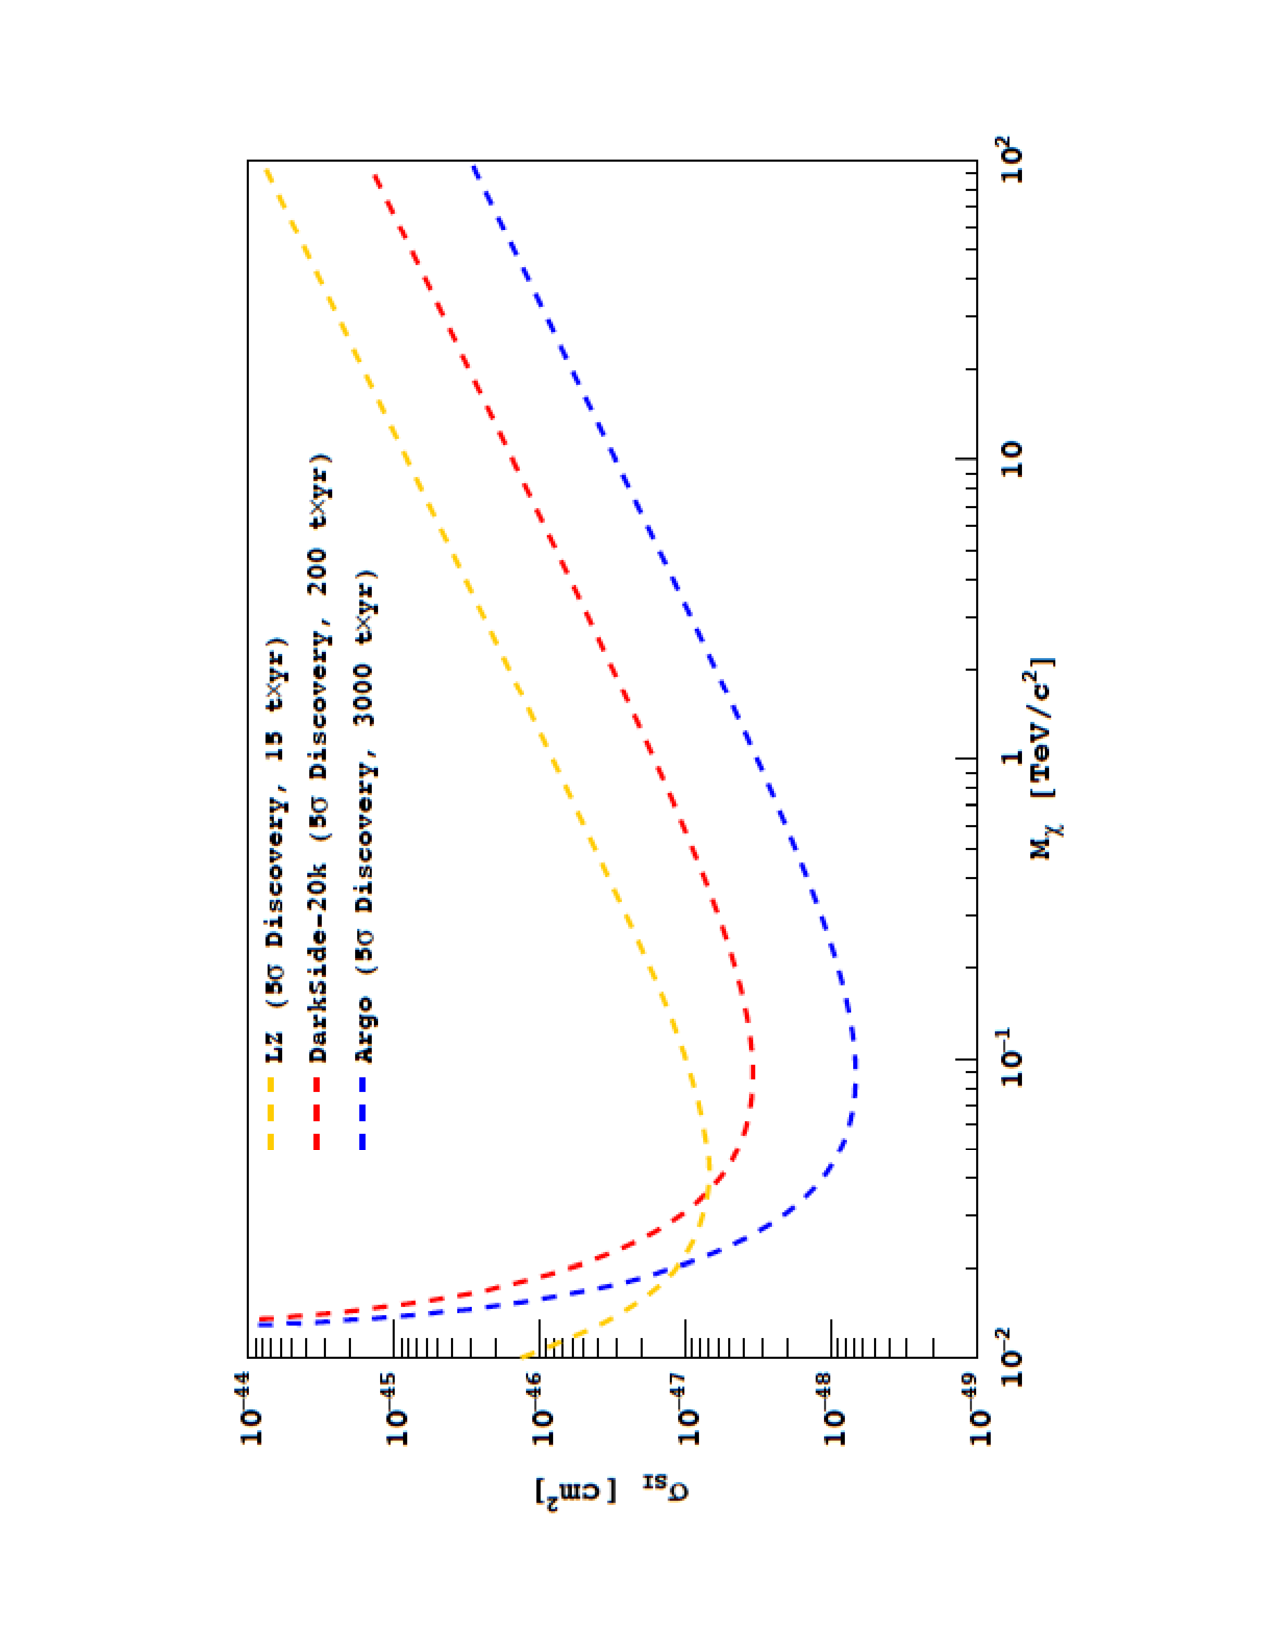
\includegraphics[width=0.65\linewidth,angle=270,origin=c]{Darkmatter/section1/img/discovery.pdf}
%  \vspace{-3.cm}
%\caption{5$\sigma$ discovery potential of the leading future noble liquid dark matter searches.}
%\label{fig:discovery}
%%
%%%%%%%%%%%%%%%%%%%%%%%%%%%%%%%%%%%
%
%

%medskip
%\noindent
%\textit{Projected sensitivities.} 
Projected sensitivities of near-future direct detection dark matter searches are shown in Fig.~\ref{fig:sensitivity} as dashed curves.  Three mid-term searches using Xe TPCs---LZ %\cite{dobsonLZ}, 
PANDA, and XENON-nT 
%\cite{grandiXENON}
---all aim to reach ~10$^{-48}$ cm$^2$ scale sensitivity at 30 GeV dark matter mass.  Searches at the HL-LHC for scalar dark matter project comparable sensitivity for the low mass range below 10~GeV,
%~\cite{futureCollider}
discussed further in Sec.~\ref{subsec:complementarity_collider}. The DarkSide-20k experiment projects reaching the 10$^{-47}$ cm$^2$ scale at 1 TeV.  Long-term future searches using Xe (DARWIN) and Ar (ARGO) project reaching beyond 10$^{-48}$ cm$^2$ in the next decade. For spin-dependent interactions, near-term future experiments using Xe and CF$_3$ targets project sensitivity to 10$^{-42}$ cm$^2$ WIMP-neutron
%~\cite{grandiXENON} 
and WIMP-proton cross sections, at $\sim$\,50 GeV.
%~\cite{sigmaSD-prospects}.
%
At low mass (around 1 to 10 GeV), solid state experiments, e.g. SuperCDMS, project 10$^{-42}$ cm$^2$ cross section reach on a 5 year time scale.

Major challenges to future direct detection experiments come from: (a)  $\nu-e$ and coherent elastic scattering backgrounds from solar and atmospheric neutrinos, which is known as the 'neutrino floor' and shown in the grey hatched region in Fig.~\ref{fig:sensitivity}; (b) neutrino flux uncertainties on these backgrounds; and, (c) technology scaling to increase in mass over current searches by factors of 10 or more whilst improving background rejection and lowering radioactivity.

% discuss complementarity in Ch.2?
%Direct detection searches have sensitivity to interactions of WIMPs with masses above the center of mass energy of the LHC, and in this way provide highly complementary reach. 
%A more detailed discussion of complementarity can be found in %~\ref{note:Support_Note_Complementarity}.
%{\bf (reference to support note)}.
In consideration of the strong synergy between direct dark matter detection and the program for its production and discovery in high-energy collisions at accelerators as well as in accelerator-based fixed target experiments, discussions at the Open Symposium in Granada highlighted that CERN's support for selected direct dark matter search programs that can take critical advantage of technology developed at CERN can deliver a decisive boost of their sensitivity.

%%%%%%%%%%%%%%%%%%%%%%%%%%%%%%%%%%
% CW: Into supporting note

%Major challenges to future experiments come from: 
%\begin{itemize}
%\item {\it Neutrino floor: } next-generation dark matter experiments will be sensitive to several sources of neutrino backgrounds, via $\nu-e$ elastic scattering and coherent elastic neutrino scattering (CE$\nu$NS) on nuclei (NR). Atmospheric and diffuse supernovae neutrinos, which due to their high energies can produce NRs in excess of 20 keVnr, will be the dominant CE$\nu$NS background contributor for WIMP masses $>$30 GeV.  Solar neutrinos are the main CE$\nu$NS background for dark matter masses $<$10 GeV.  
%
%\item {\it Neutrino flux uncertainties: }
%%
%in addition to astrophysical uncertainties~\cite{Green:2017odb}, when calculating the discovery sensitivity of a dark matter search experiment, one must also fully account for the uncertainties on neutrino-induced backgrounds. The 'neutrino floor' (shown as the grey hatched region in Fig.~\ref{fig:sensitivity}), initially conceived as indicative of the maximum sensitivity attainable in the presence of CE$\nu$NS background, depends critically on the target, experimental technique, statistical analysis, neutrino flux and cross section uncertainties.  Fig.~\ref{fig:discovery} includes a detailed accounting of the CE$\nu$NS and $\nu-e$ backgrounds in the sensitivity and discovery potential. A 20\% uncertainty on the neutrino background for high-mass ($>$30 GeV) searches is assumed; to account for a 15\% uncertainty on the atmospheric neutrino flux at mid-latitude locations, such as LNGS, based on the latest data-driven models of cosmic primaries \cite{PhysRevD.95.023012} as well as models of solar
%cycle, seasonal, geographic, and geomagnetic dependence of the neutrino flux~\cite{PhysRevD.83.123001,PhysRevD.74.094009}. The theoretical uncertainty on the Standard Model interaction cross-section is assumed to be 5\%, driven by uncertainties on the nuclear form factor and the expected constraints that the COHERENT collaboration will place on non-Standard Model contributions using a LAr target \cite{Akimov1123}.
%%which in turn is driven by their current 10\% uncertainty on neutrino flux \cite{Tayloe_2018} and a 6\% uncertainty on the LAr response as measured by SCENE \cite{PhysRevD.91.092007, PhysRevD.88.092006} and ARIS \cite{PhysRevD.97.112005}. 
%%Planned improvements of COHERENT, including a sharper characterization of the neutrino  flux and a measurement with a LAr target, would further reduce the uncertainty on the neutrino background below 10\%, strongly benefitting the DarkSide experiments. \\
%
%\item {\it Technology Scaling:} 
%%
%If dark matter cross sections are below the reach of near-future experiments, detectors must increase in mass over current and near-future searches by factors of 10 or more to discover dark matter at 5$\sigma$, or to test whether new particles discovered at the LHC above a few GeV make up the galactic dark matter halo. The DARWIN experiments plans a 30-50 t Xe TPC, and the ARGO experiment aims for a 400 t Ar target (reach shown in Fig.`\ref{fig:discovery}).  At this scale new technology solutions are required, leading to collaboration with HEP around areas of mutually beneficial technology development, for example in cryostat technology and Si-detector based photon sensing.
%%
%%Given the cost of the target and the onset of neutrino-electron scattering backgrounds, LAr detectors are the only feasible strategy towards kilotonne-scale dark matter detectors. 
%
%\end{itemize}
%
%
%The existence of dark matter, and its role in shaping the formation of our Universe, is an important signpost towards new physics extending beyond the Standard Model of Particle Physics and provides strong rationale for an aggressive program of exploration for new physics at both the energy frontier and the low-background frontier.  Today, searches for dark matter at accelerators and via direct detection experiments are at the forefront of the exploration of the dark sector of physics.  The exploration of dark matter through all avenues will cross-fertilize the program of searches at accelerators and could provide important directions for the development of future, large-scale facilities.  In the meanwhile, as direct dark matter detectors start approaching significant issues related to their scaling in mass and sensitivity, the role of technology developed a CERN in enabling the next generation of discovery tools comes more than ever into sharp focus.  
%
%In consideration of the strong synergy between direct dark matter detection and the program for its production and discovery in high-energy collisions at accelerators, CERN's support for selected direct dark matter search programs that can take critical advantage of technology developed at CERN can deliver a decisive boost of of their sensitivity.

%%
%%%%%%%%%%%%%%%%%%%%%%%%%%%%%%%%%%%%%%%%%%%%

%\newpage

\subsection{Indirect detection}

Indirect astrophysical searches for the annihilation products of dark matter (namely gamma-rays, neutrinos, anti-matter) provide important and complementary constraints on dark matter models that are searched for at particle colliders and fixed target/beam dump experiments, as well as on models with axion-like particles.   Annihilation searches are sensitive to the thermal cross-section for dark matter masses up to 100 GeV (depending on the channel), with prospects to reach 10 TeV within less than ten years.  No conclusive signals have been found so far.

\begin{figure}
    \centering
    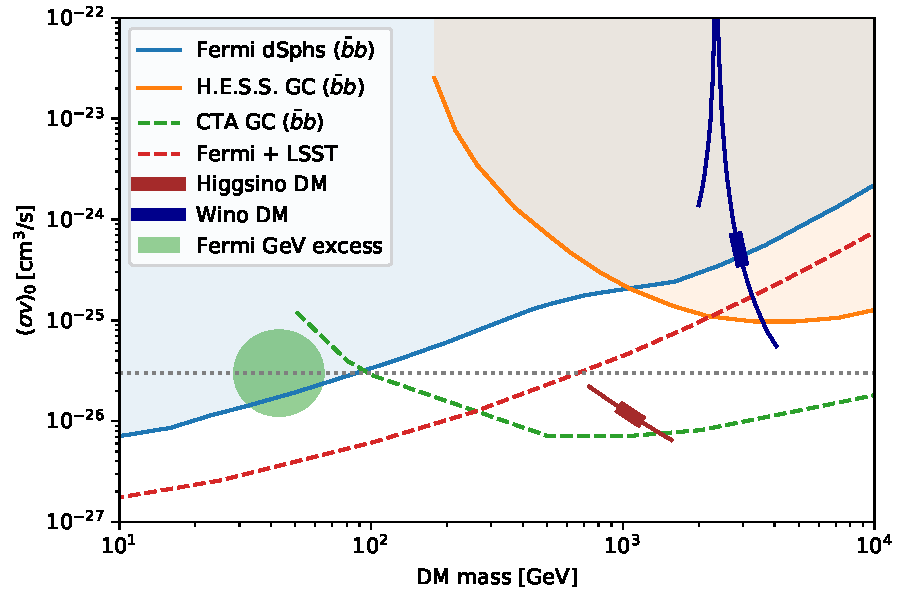
\includegraphics[width=0.8\linewidth]{Darkmatter/section1/img/ID.pdf}
    \caption{Current constraints on the dark matter self-annihilation cross-section into $\bar bb$ from Fermi LAT (dSph)~\cite{Albert2017-hn} and H.E.S.S.~Galactic Centre (GC)~\cite{Abdallah:2016ygi}, and expected future reach with the CTA and additional dwarfs found by LSST~\cite{Drlica-Wagner:2019xan}. 
    %Constraints on other hadronic final two-body states differ typically within a factor of less than two. 
    Also shown as red (blue) lines the annihilation cross-sections for pure Higgsino (Wino) DM (with thick regions indicating correct relic density, from~\cite{Ibe:2015tma}), as well as the parameter range preferred by the Fermi GeV excess~\cite{Ackermann:2017gx, Albert2017-hn}. The H.E.S.S.~constraints weaken significantly if the DM profile at the Galactic center is cored, leaving pure Wino DM consistent with H.E.S.S.~and Fermi observations (see text for details).}%~\cite{Cohen2013-ah, Cabrera-Catalan2015-os, %Hryczuk2019-mv}
    %Crosses indicate the pure Wino and Higgsino cases, respectively~\cite{Cabrera-Catalan2015-os}.} 
    \label{fig:ID}
\end{figure}

The arguably cleanest constraints on DM annihilation in the GeV--TeV mass range come from gamma-ray observations of dwarf spheroidal (dSph) galaxies. Recent analyses (based on a few dozens of dSphs) exclude s-wave annihilating WIMPs into $\bar b b$ with masses between 5 and 80 GeV~\cite{Albert2017-hn} (Fig.~\ref{fig:ID}).  The arguably best example for a DM annihilation signal \emph{candidate} is the so-called `Fermi GeV excess'~\cite{Ackermann2017-gy}, an excess emission of GeV photons in the inner Galaxy.  It is marginally consistent with dSph and anti-proton constraints.  Astrophysical interpretations of the excess will be probed with upcoming radio observations (millisecond pulsar searches~\cite{Calore:2015bsx}), while collider experiments can test the dark matter origin.  For instance, if interpreted in terms of 60 GeV dark matter in supersymmetric models (consistent with dSphs, see Fig.~\ref{fig:ID}), the decays of heavy CP-odd and CP-even scalars into $\tau$-pair provides a possible target for the HL-LHC~\cite{Carena:2019pwq}.  In a simple model with a scalar mediator and fermionic Dirac DM with $\bar bb$ annihilation channel, effects on the Higgs signal strength and exotic Higgs decay can be probed with prospective future colliders such as  ILC and FCC-hh~\cite{Kim2018-yk}.  Furthermore, DM annihilation into $\bar bb$ or other hadronic final states contribute significantly to the cosmic-ray anti-nuclei flux observed at Earth~\cite{Giesen:2015ufa}. Future probes of DM annihilation into hadronic final states (sensitive to the Fermi GeV excess), will come from anti-deuteron measurements with the balloon experiment GAPS (around 2021) and AMS-02~\cite{Aramaki2016-to}.

The future LSST has the potential to discover hundreds of additional dSphs~\cite{Drlica-Wagner:2019xan}, which together with Fermi LAT data can improve limits from dSph galaxies by a factor of around five.  The upcoming Cherenkov Telescope Array (CTA) is expected to strengthen current H.E.S.S.~constraints by a factor about ten~\cite{Drlica-Wagner2019-nr, Carr2016-vl}, see Fig.~\ref{fig:ID}.
%for current limits compared with future reach in the $\bar bb$ final state.  Note that constraints on other hadronic final two-body states differ typically within a factor of less than two.
%
% JRM:  moved this to section 2.2 on complementarity as discussed 7.16.19
%Above about 0.5--1 TeV DM mass, observations of the inner Galaxy with the Cherenkov Telescope H.E.S.S.~start to provide the strongest constraints on dark matter annihilation, almost reaching the thermal cross-section~\cite{Abdallah:2016ygi}.   Pure Wino dark matter with a mass around 3 TeV~\cite{Beneke:2016ync}, which would account for all of dark matter, is constrained by these searches if the dark matter distribution at our Galactic center has a cusp-like profile~\cite{Cohen2013-ah, Cabrera-Catalan2015-os, Hryczuk2019-mv}.  
%However, if the distribution is more cored, the constraints become weaker. Wino dark matter can also be probed with the FCC-hh~\cite{CidVidal:2018eel}, while lighter Wino-like dark matter would be already accessible for HE-LHC~\cite{CidVidal:2018eel} and CLIC$_{3000}$~\cite{deBlas:2018mhx}.The future Cherenkov Telescope Array (CTA) will improve on current H.E.S.S.~constraints by another order of magnitude~\cite{Drlica-Wagner2019-nr, Carr2016-vl, Silverwood2015-ff}.  In the case of a discovery, the combination of CTA and collider results would allow to determine the dark matter distribution at the galactic center precisely, with important implications for the formation history and evolution of galaxies.
%%This could have a  big impact on our understanding of the evolution of galaxies and the massive black hole in our galactic center. CTA will be furthermore sensitive to Higgsino dark matter with a mass about $1.1$ TeV~\cite{Cabrera-Catalan2015-os, Krall:2017xij, Hryczuk2019-mv}, which is also a target of the FCC-hh~\cite{CidVidal:2018eel} and CLIC$_{3000}$~\cite{deBlas:2018mhx}.  Interestingly, many of these models would be below the neutrino floor of direct searches, emphasizing the complementarity between the experimental approaches.
%
Furthermore, neutrino observations of the Sun with IceCube/ANTARES %~\cite{Adrian-Martinez2016-yb, IceCube_Collaboration2016-fp} 
provide in many cases the most stringent constraints on the spin-dependent WIMP-proton cross-section.  The ORCA detector of KM3NeT and the IceCube Upgrade are expected to further probe spin-dependent cross-sections down to $3\times10^{-5}\,\text{pb}$, for dark matter masses below $\sim 100$ GeV.
%~\cite{Backstrom:2018plo, Coyle2017-cj, PhysRevLett.114.141301, Aartsen:2017ulx, Chen_2014}.
These ranges will also be probed by upcoming direct detection experiments~\cite{sigmaSD-prospects}.




%Recently, a discussion started about a possible excess of anti-protons at around 15 GV~\cite{Cuoco2017-tc, Reinert2018-et, Cholis2019-zx, Cuoco2019-hu}.  When interpreted in terms of a dark matter annihilation signal, it is consistent the parameters required for the Fermi GeV excess. 

%Searches with the existing MeerKAT radio telescope 
%array have the potential to find the radio-brightest of the MSPs in the
%upcoming years~\cite{Calore2016-td}. 
%However, there is still no consensus and the discussion has been recently
%revived in ref.~\cite{XXX}.  




%\subsection{Guidelines}
%
%The main repository of the report material is Overleaf. If you are not
%registered with Overleaf as yet, you can do so. Use your cern.ch mail
%account, as this will give you, for free, the Professional license. This
%is needed if you want to access the full functionality, including the
%ability to grant editing rights to many people.
%
%You can create the project for your section by just cloning this
%project. It's important that you do it using your professional
%Overleaf account (namely with your cern.ch email credentials), since
%the project inherits the functionalities available to its owner.
%After creating the project, make sure you set the proper
%administration rights, listing people who will have editing
%rights. You can do this clicking on the "share" button on top of the overleaf project page. You are given various options, such as making the project read/write accessible to anyone who has the url, or just readable to anyone who has a (different) url, or restricted to users selected in a list. The same button gives you the git repository url, to download the project locally. Notice that those you give rights to cannot further assign
%rights to others. Only the owner of the project can grant access
%rights. Of course section editors can clone a new version of the whole
%chapter, leave alone the other sections to focus on their own, and
%grant access to it to their co-editors. At the end they just put
%things back into the master project.  I understood that it should be
%possible to grant rights to a CERN e-group, but I am not sure this is
%working already, I'm waiting for confirmation.
%
%You can work directly on the Overleaf version, or you can download the
%whole package locally from the git repository. You can then use the
%standard git tools to commit updated versions. Working locally is
%almost essential at the beginning of the project, when you want to
%create a complete subfolder structure to contain the various sections
%of your report. Some scripts are available (see below) to faciliate
%this task.
%
%This document can be compiled in its entirety, using the\\
%$>$ pdflatex report\\
%command from the main directory. In alternative, you can compile
%individual sections, with the command\\
%$>$ pdflatex section\\
%issued from the section subdirectory. This will generate the complete
%section, including its 
%bibliography.
%I am not sure this is possible when working directly on the web with
%Overleaf. But this works in your local version, if you input the
%pdflatex commands yourself.
%
%For this to work, you must preserve the template
%structure of the section.tex file in the directory of each
%section. You should also make sure that all style files contained in
%the main directory are present in the section directories. The
%simplest way to create a new section is to issue the command
%\begin{verbatim}
%> make newsection newfolder=new_folder_name
%\end{verbatim}
%from the main directory. Here \verb|new_folder_name| is the name of the
%directory you want to create to host the new section. A template section
%file will be created there, together with the img and bib directories
%(for figures and for the section.bib file, resp).
%All necessary style files are copied over. Now you just need to input
%the \verb|new_folder_name/section.tex| file into the main driver file,
%report.tex, with the syntax:
%\begin{verbatim}
%\newpage
%\subfile{\main/newdirectory/section}
%\end{verbatim}
%When editing the new \texttt{section.tex} file, please pay attention to the
%header of the template. There are a few weirds commands, and an
%apparently odd
%\verb|\begin{document}|
%statement. These are required to be able to compile the section as a
%stand alone object. To this end, it is important that the command
%\verb|\providecommand{\main}{..}|
%points \verb|\main| to the directory containing the main driver file,
%\texttt{report.tex}. The file paths to figures
%(Fig.~\ref{fig:higgs}) must all include this absolute
%reference, as in
%\begin{verbatim}
%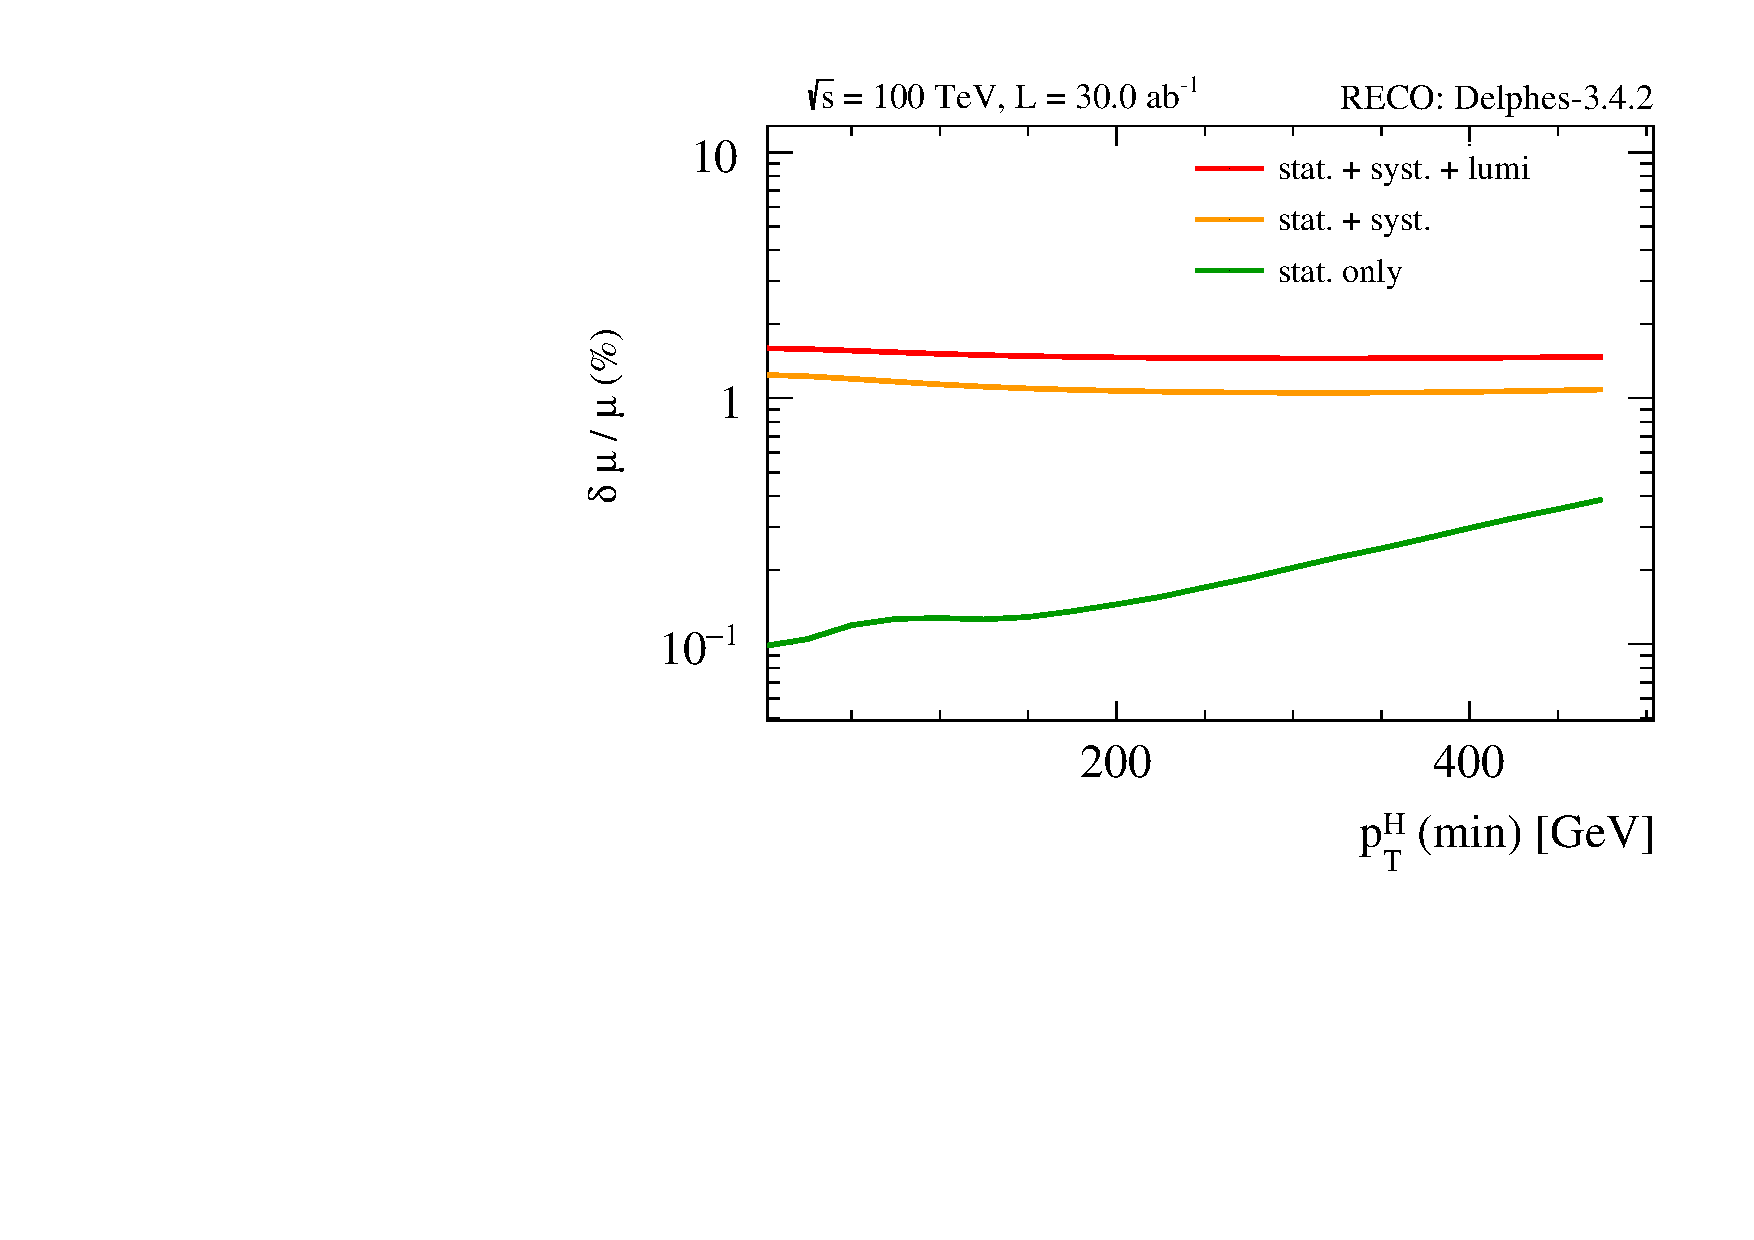
\includegraphics[width=0.45\textwidth]{\main/Darkmatter/section1/img/hgg.pdf} .
%\end{verbatim}
%
%\begin{figure}[ht]
%\centering
%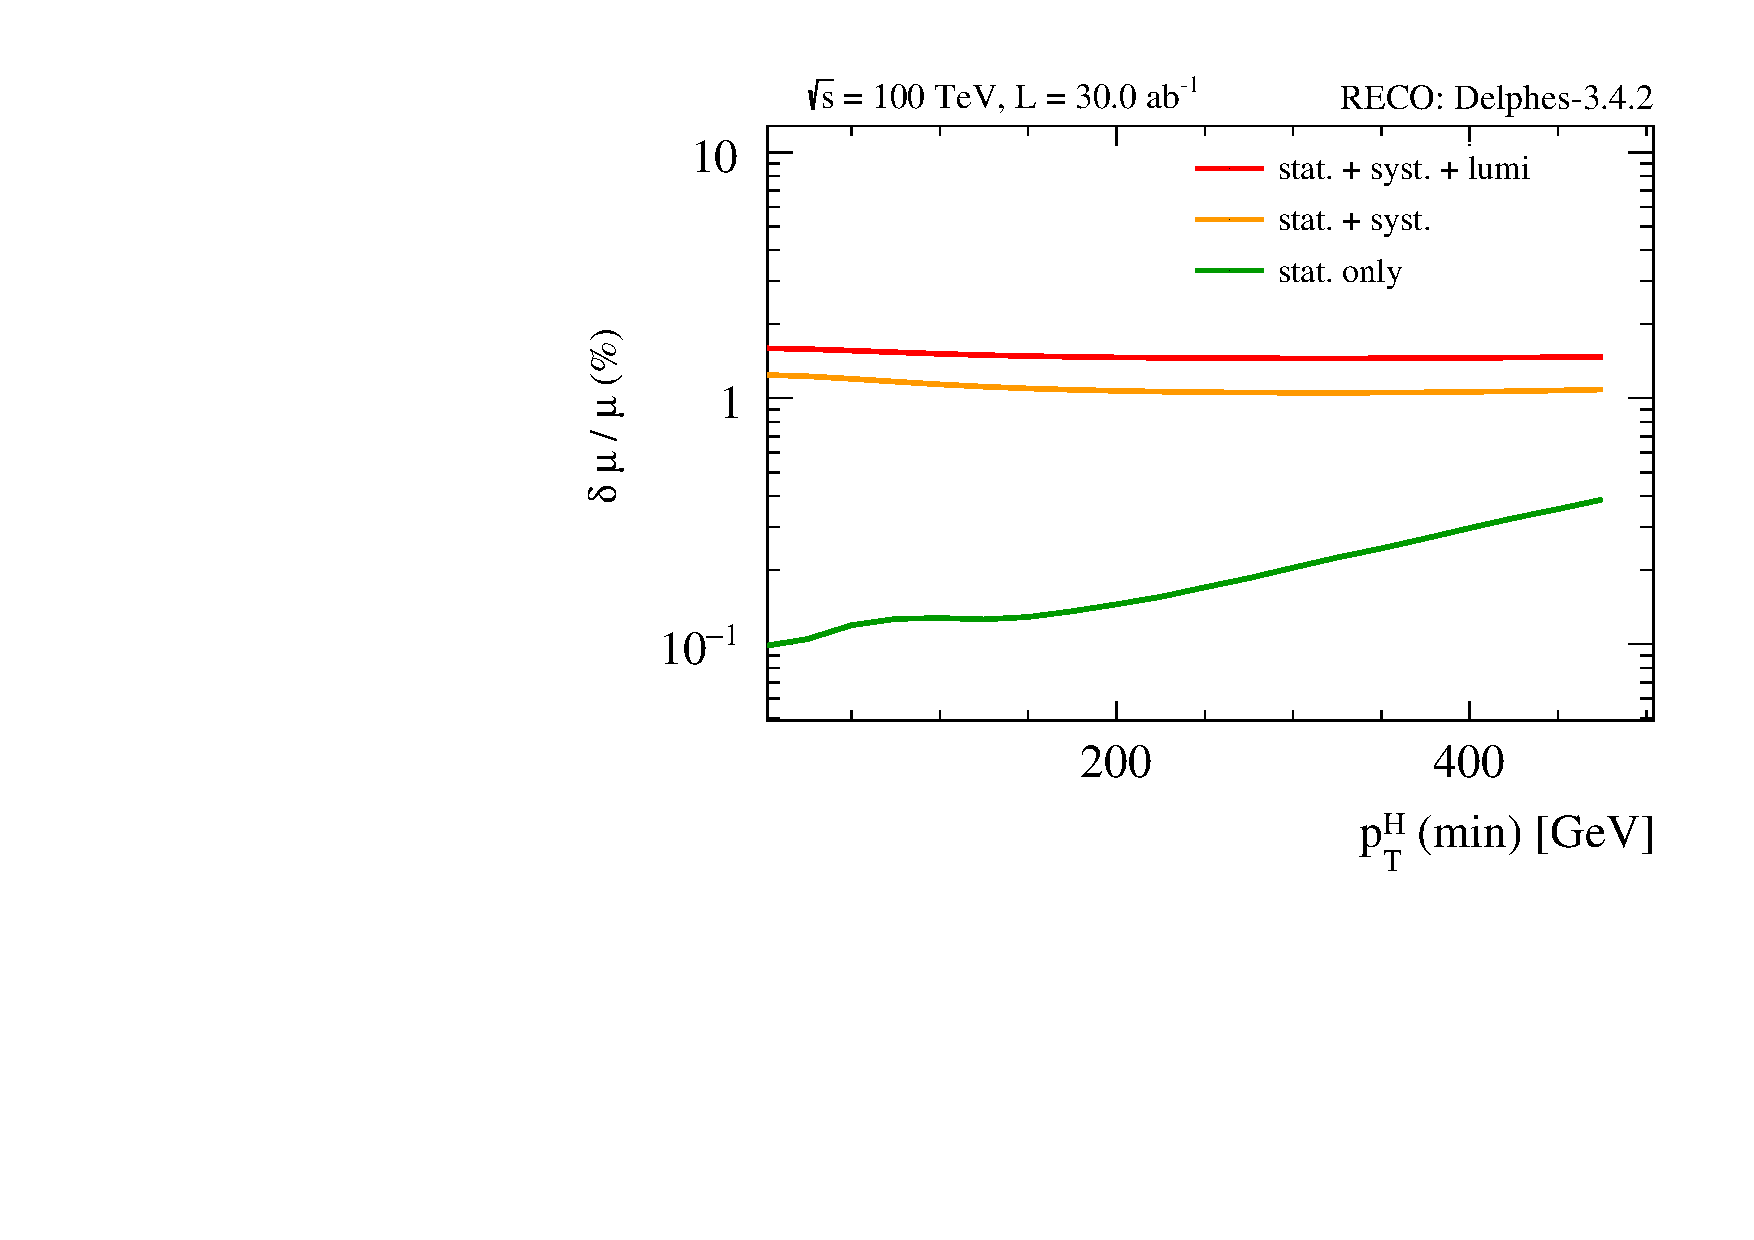
\includegraphics[width=0.75\textwidth]{\main/Darkmatter/section1/img/hgg.pdf}
%\caption{Caption of the figure.}
%\label{fig:higgs}
%\end{figure}
%
%As for tables, please use the standard tabular environment, with the
%caption on top of the table. For cross referencing, try use lables
%such as
%\verb|\label{eq:eqname}|, \verb|\label{tab:tabname}| and
%\verb|\label{fig:figname}|. 
%
%If you need subsections, you can include them here directly, or input
%them as files, which can live in their own subdirectory. If including
%a subsection from a file, import them with the command
%\begin{verbatim}
%\subfile{\main/Darkmatter/section1/sub1/mysubsec}
%\end{verbatim}
%where mysubsec.tex would start of course with the statement
%\verb|\begin{subsection}|.  In this case, make sure you define
%properly the path to figures and other files. This is crucial to
%guarantee compatibility of compilation of the whole Chapter and or the
%individual section. The fact that a Section compiles doesn't imply
%that the Chapter will compile, if paths are entered inaccurately. At
%this time I have not foreseen the ability to compile subsections
%standalone, I hope it is not necessary.
%
%We defined some small macros to allow comments to be made. F`or instance \BH{this is a comment by Beate}.

%
%\subfile{\main/Darkmatter/section1/sub1/mysubsec}

%\CW{N64 and SENSEI complementarity. 1807.03790}
%\CW{Check out Cid Vidal X}
%\CW{Fig: 2, extract blobs from Fig. 2 1905.00315}
%\CW{Check section 2, add bullets}

% From JM
%Data from the PAMELA satellite-borne experiment show a positron excess in the cosmic rays with dark matter annihilation suggested as a possible cause \cite{Adriani:2009ci}. The Alpha Magnetic Spectrometer (AMS) measurements of the primary cosmic-ray electron and positron fluxes require more than a single power-law spectrum to be correctly described, and while this constrains some dark matter annihilation channels, it still leaves others viable \cite{Aguilar:2014cj}. The Fermi Large Area Telescope measures an emission from the Galactic center that is not fully described by background models \cite{Ackermann:2017gx}, which has been suggested to be from dark matter annihilation \cite{Ajello:2016ge}.  The near-future Cherenkov Telescope Array is sensitive to photons from annihilating dark matter in the inner Milky Way and dwarf galaxies, up to 10 TeV mass \cite{carr_1508.06128}.

%Indirect detection (ID) of dark matter aims at identifying signatures of
%non-gravitational energy transfer from the dark into the visible sector.  The
%most relevant transfer mechanisms are the self-annihilation, decay or
%oscillation of DM into particles of the standard model.  We concentrate here on
%ID of WIMP annihilation, but emphasize that also DM decay or oscillation can be
%connected to signatures at particle colliders (see additional notes).

%Searches make slow but steady progress, typically at the rate of around one decade in liftime/annihilation rate per decade.  

%- In particular for dark matter masses below $\sim100$ GeV, various searches exclude s-wave annihilating WIMP dark matter. 

%- There is a tight connection between the observed DM density and the annihilation cross-section today, which implies that $(\sigma v)_0 \simeq 3\times10^{-26}\text{cm}^3\text{s}^{-1}$. 


%Ongoing and future experiments become increasingly sensitive to this value.
%However, it is useful to keep in mind that in complete theoretical models for
%WIMP DM, the cross-section today can vary over many order of magnitudes,
%depending on the relevance of co-annihilation, resonances and kinematic
%thresholds for the annihilation in the early Universe.  This makes the direct
%comparison with other DM searches model-dependent (see notes for additional
%information).

%The exact numerical value of the constraints depends on the particular combination of dSphs included, and details of the modeling of DM in dSph (e.g.,~\cite{Hoof2018-wv}).

%For cuspy DM profiles, they reach almost the thermal cross-section (assuming $\bar bb$ final states).

\end{document}
